% Name: Unit circle
% Description: An angle θ on the unit circle with its cosine and sine drawn as the legs of a right triangle.
% Tags: unit circle, trigonometry, sine, cosine

\usetikzlibrary{arrows.meta}

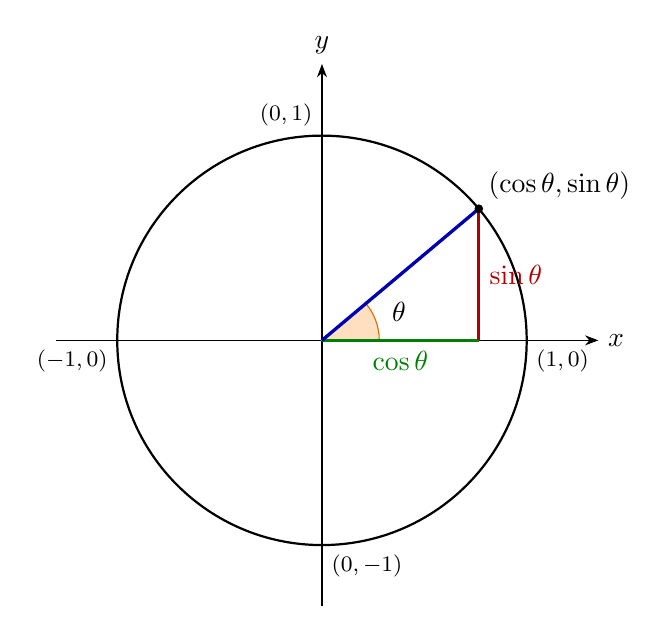
\begin{tikzpicture}[scale=2.6, >={Stealth}]
  \coordinate (P) at (40:1);
  \draw[->] (-1.3,0) -- (1.35,0) node[right] {$x$};
  \draw[->] (0,-1.3) -- (0,1.35) node[above] {$y$};
  \draw[thick] (0,0) circle (1);
  \draw[fill=orange!25, draw=orange!85!black] (0,0) -- (0.28,0) arc[start angle=0, end angle=40, radius=0.28] -- cycle;
  \node at (20:0.4) {$\theta$};
  \draw[very thick, green!50!black] (0,0) -- node[below] {$\cos\theta$} (P |- 0,0);
  \draw[very thick, red!70!black] (P |- 0,0) -- node[right] {$\sin\theta$} (P);
  \draw[very thick, blue!70!black] (0,0) -- (P);
  \fill (P) circle (0.6pt) node[above right] {$(\cos\theta, \sin\theta)$};
  \foreach \a/\label/\pos in {0/{(1,0)}/below right, 90/{(0,1)}/above left, 180/{(-1,0)}/below left, 270/{(0,-1)}/below right}
    \node[font=\footnotesize, \pos] at (\a:1) {$\label$};
\end{tikzpicture}
